% Filo-Priori Framework Overview Figure
% Compile with: pdflatex fig_framework_overview.tex
\documentclass[tikz,border=2pt]{standalone}
\usepackage{tikz}
\usetikzlibrary{shapes.geometric, arrows.meta, positioning, fit, backgrounds, calc, decorations.pathreplacing}
\usepackage{xcolor}

% IEEE-style colors
\definecolor{ieeeblue}{RGB}{0,84,147}
\definecolor{ieeelightblue}{RGB}{200,220,240}
\definecolor{ieeegreen}{RGB}{0,128,0}
\definecolor{ieeeorange}{RGB}{230,159,0}
\definecolor{ieeegray}{RGB}{128,128,128}
\definecolor{inputcolor}{RGB}{255,245,230}
\definecolor{processcolor}{RGB}{230,245,255}
\definecolor{outputcolor}{RGB}{230,255,230}

\begin{document}
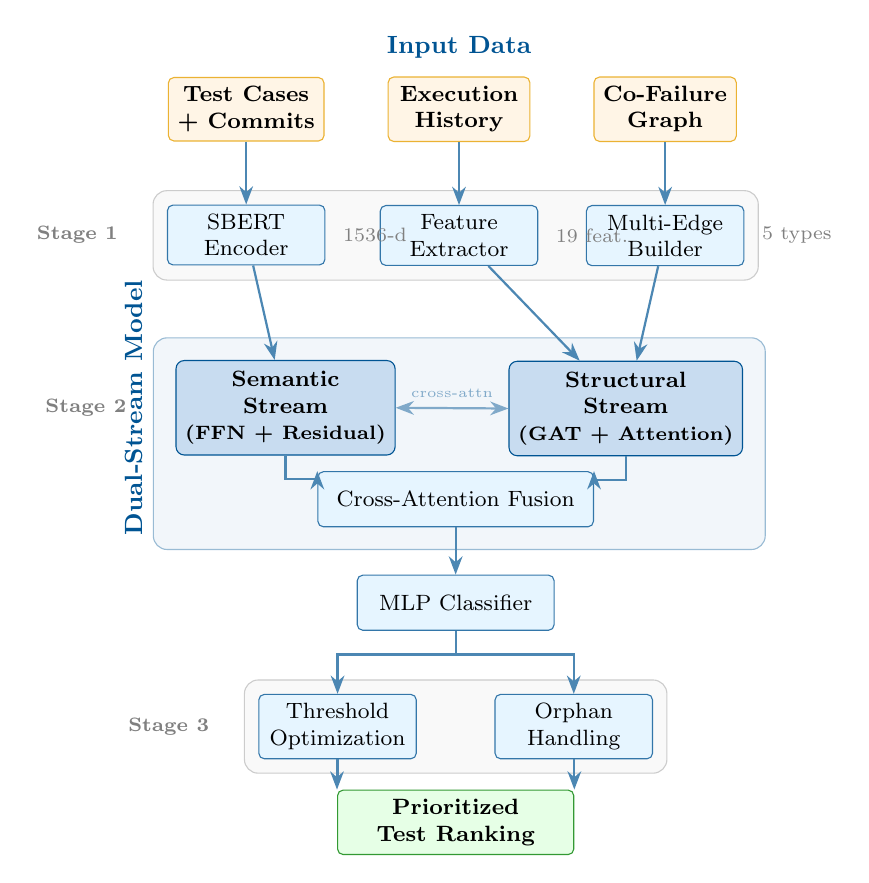
\begin{tikzpicture}[
    node distance=0.4cm and 0.6cm,
    >=Stealth,
    every node/.style={font=\footnotesize},
    inputbox/.style={rectangle, draw=ieeeorange!80, fill=inputcolor,
        minimum width=1.8cm, minimum height=0.7cm, rounded corners=2pt,
        align=center, font=\footnotesize\bfseries},
    processbox/.style={rectangle, draw=ieeeblue!80, fill=processcolor,
        minimum width=2cm, minimum height=0.7cm, rounded corners=2pt,
        align=center},
    modulebox/.style={rectangle, draw=ieeeblue, fill=ieeelightblue,
        minimum width=2.4cm, minimum height=1.2cm, rounded corners=3pt,
        align=center, font=\footnotesize\bfseries},
    outputbox/.style={rectangle, draw=ieeegreen!80, fill=outputcolor,
        minimum width=2cm, minimum height=0.7cm, rounded corners=2pt,
        align=center, font=\footnotesize\bfseries},
    arrow/.style={->, thick, ieeeblue!70},
    dashedarrow/.style={->, thick, dashed, ieeegray},
    label/.style={font=\scriptsize, ieeegray},
]

% === INPUT SECTION ===
\node[inputbox] (testdata) {Test Cases\\+ Commits};
\node[inputbox, right=0.8cm of testdata] (history) {Execution\\History};
\node[inputbox, right=0.8cm of history] (graph) {Co-Failure\\Graph};

% === FEATURE EXTRACTION ===
\node[processbox, below=0.8cm of testdata] (sbert) {SBERT\\Encoder};
\node[processbox, below=0.8cm of history] (features) {Feature\\Extractor};
\node[processbox, below=0.8cm of graph] (graphbuild) {Multi-Edge\\Builder};

% Dimensions
\node[label, right=0.1cm of sbert] {1536-d};
\node[label, right=0.1cm of features] {19 feat.};
\node[label, right=0.1cm of graphbuild] {5 types};

% === DUAL-STREAM MODEL ===
\node[modulebox, below=1.2cm of sbert, xshift=0.5cm] (semantic) {Semantic\\Stream\\{\scriptsize (FFN + Residual)}};
\node[modulebox, below=1.2cm of graphbuild, xshift=-0.5cm] (structural) {Structural\\Stream\\{\scriptsize (GAT + Attention)}};

% Cross-attention
\node[processbox, below=0.8cm of $(semantic)!0.5!(structural)$, minimum width=3.5cm] (crossattn) {Cross-Attention Fusion};

% === CLASSIFICATION ===
\node[processbox, below=0.6cm of crossattn, minimum width=2.5cm] (classifier) {MLP Classifier};

% === POST-PROCESSING ===
\node[processbox, below=0.8cm of classifier, xshift=-1.5cm] (threshold) {Threshold\\Optimization};
\node[processbox, below=0.8cm of classifier, xshift=1.5cm] (orphan) {Orphan\\Handling};

% === OUTPUT ===
\node[outputbox, below=0.8cm of $(threshold)!0.5!(orphan)$, minimum width=3cm] (output) {Prioritized\\Test Ranking};

% === ARROWS ===
% Input to extraction
\draw[arrow] (testdata) -- (sbert);
\draw[arrow] (history) -- (features);
\draw[arrow] (graph) -- (graphbuild);

% Extraction to streams
\draw[arrow] (sbert) -- (semantic);
\draw[arrow] (features) -- (structural);
\draw[arrow] (graphbuild) -- (structural);

% Streams to fusion
\draw[arrow] (semantic.south) -- ++(0,-0.3) -| (crossattn.north west);
\draw[arrow] (structural.south) -- ++(0,-0.3) -| (crossattn.north east);

% Bidirectional cross-attention indicator
\draw[<->, thick, ieeeblue!50] (semantic.east) -- (structural.west)
    node[midway, above, font=\tiny] {cross-attn};

% Fusion to classifier
\draw[arrow] (crossattn) -- (classifier);

% Classifier to post-processing
\draw[arrow] (classifier.south) -- ++(0,-0.3) -| (threshold.north);
\draw[arrow] (classifier.south) -- ++(0,-0.3) -| (orphan.north);

% Post-processing to output
\draw[arrow] (threshold.south) -- ++(0,-0.3) -| (output.north west);
\draw[arrow] (orphan.south) -- ++(0,-0.3) -| (output.north east);

% === ANNOTATIONS ===
% Input label
\node[above=0.1cm of history, font=\small\bfseries, ieeeblue] {Input Data};

% Model label
\node[left=0.3cm of semantic, font=\small\bfseries, ieeeblue, rotate=90, anchor=south] {Dual-Stream Model};

% Background boxes
\begin{scope}[on background layer]
    \node[draw=ieeegray!40, fill=gray!5, rounded corners=5pt,
          fit=(sbert)(graphbuild), inner sep=5pt] {};
    \node[draw=ieeeblue!40, fill=ieeeblue!5, rounded corners=5pt,
          fit=(semantic)(structural)(crossattn), inner sep=8pt] {};
    \node[draw=ieeegray!40, fill=gray!5, rounded corners=5pt,
          fit=(threshold)(orphan), inner sep=5pt] {};
\end{scope}

% Stage labels
\node[label, left=0.5cm of sbert] {\textbf{Stage 1}};
\node[label, left=0.5cm of semantic] {\textbf{Stage 2}};
\node[label, left=0.5cm of threshold] {\textbf{Stage 3}};

\end{tikzpicture}
\end{document}
